\section{Session Date: 3rd January, 2025}
\subsection*{Main Topic: Electromagnetism}
\subsection*{Topics Covered: Ch. 10 Griffiths}
\begin{itemize}
    \item Solution to the four-dimensional wave-equation
    \item Liénard-Wiechert potentials
    \item Fields from a moving point charge
\end{itemize}

\subsection*{Notes}
\subsubsection*{Idea: Potential Formulation of Electrodynamics}
The goal of Chapter 10 in Griffiths is to find a general solution to Maxwell's equations in terms of potentials (we are working in the Lorenz Gauge). The very central thing to keep in mind is that information travels at the speed of light, such that the potential at some distance \(\griffr[2]\) isn't given by the source distributions at some time \(t\), but rather at the retarded time (dependent on the distance to the source) \begin{align*}
    \boxed{t_r = t - \frac{\griffr[2] }{c}}\tag{10.25}
\end{align*}

By finding the solution to Maxwell's equations in the potential formulation 
\begin{align*}
    &\square^{2} V(\mathbf{r}, t) = - \frac{1}{\epsilon _0} \rho (\mathbf{r}, t)\\
    &\square^{2} \mathbf{A}(\mathbf{r}, t) = -\mu _0 \mathbf{J}(\mathbf{r}, t)
\end{align*}
we can subsequently calculate the fields. But since the relevant \textit{time} now depends on position (space-time), differentiating sources is non-trivial. And this even applies to point charges. This is because classical electrodynamics formulates sources in terms of densities, and as such we have to define the densities related to point charges as the density of a charge with finite extension as the size goes to zero. It seems weird that there can be different retarded times from the same field point to a point charge, but that's apparently necessary with classical electrodynamics. 

\subsubsection*{The Generalized Potentials}
We have already found solutions for electro\textit{statics} (with the Coloumb Gauge) \begin{align*}
    V(\mathbf{r}) &= \frac{1}{4\pi\epsilon_0} \int \frac{\rho (\mathbf{r}^{\prime} )}{\griffr[2] } d \tau ^{\prime}\\
    \mathbf{A}(\mathbf{r}) &= \frac{\mu_0}{4 \pi } \int \frac{\mathbf{J}(\mathbf{r}^{\prime} )}{\griffr[2]} d \tau ^{\prime} 
\end{align*}
The naïve idea is to just make the transition \begin{align*}
    &\rho (\mathbf{r}^{\prime} ) \to \rho (\mathbf{r}^{\prime}, t)\\
    &\mathbf{J}(\mathbf{r}^{\prime} ) \to \mathbf{J}(\mathbf{r}^{\prime}, t)
\end{align*}
BUT, since the fields can maximally communicate at the speed of light, the sources should not be evaluated at some global time \(t\), but rather we should evaluate them at the \textit{retarded} time:
\begin{align*}
    t_r = t - \frac{\griffr[2] }{c}
\end{align*} 
which means that any field point "sees" the charge distribution at a different time depending on the radial distance from the source (and as such there are in fact infinitely many retarded times, dependent on the relative distance). It turns out that the generalisation of Maxwell's equations in terms of retarded potentials in fact is just the naïve potentials, but with the retarded times instead \begin{align*}
    \boxed{V(\mathbf{r}, t) = \frac{1}{4\pi\epsilon_0} \int \frac{\rho (\mathbf{r}^{\prime}, t_r )}{\griffr[2] } d \tau ^{\prime}, \qquad \mathbf{A}(\mathbf{r}, t) = \frac{\mu_0}{4 \pi } \int \frac{\mathbf{J}(\mathbf{r}^{\prime}, t_r)}{\griffr[2]} d \tau ^{\prime}} \tag{10.26}
\end{align*}
Notice how we on the left have find the potential at the point \(\mathbf{r}\) at the time \(t\), whereas we on the right have the source point \(\mathbf{r}^{\prime} \)  and the retarded time \(t_r\). But since this is integrated away, we end up with the correct dependencies. Since every field point sees the source point at a distinct retarded time (depending on radial distance) it does not seem so out of touch to think about \((\mathbf{r}^{\prime}, t_r)\) as a coordinate in 4 dimensions without making the time coordinate too special. We can already see how a "native relativistic" formulation of these equations could be quite elegant.

This can directly be showed to solve Maxwell's equations \begin{align*}
    &\square^{2} V(\mathbf{r}, t) = - \frac{1}{\epsilon _0} \rho (\mathbf{r}, t)\\
    &\square^{2} \mathbf{A}(\mathbf{r}, t) = -\mu _0 \mathbf{J}(\mathbf{r}, t)
\end{align*}
just by taking the gradient and then the divergence. 
\subsubsection*{Mathematical Takeaways}
\paragraph{Remember the chain rule!}
Some takeaways from that derivation is \begin{align*}
    \nabla \left( \frac{\rho (\mathbf{r}^{\prime} , t_r)}{\griffr[2] } \right) &= \partial  _i \left( \frac{\rho (\mathbf{r}, t_r)}{\griffr[2] } \right)\\
    &= \frac{1}{\griffr[2] }\partial  _i \rho + \rho \partial_i \left( \frac{1}{\griffr[2] } \right) \\
    &= \frac{1}{\griffr[2] }\frac{\partial \rho}{\partial t} \frac{\partial t}{\partial t_r} \frac{\partial t_r}{\partial x_{i} }  - \rho \frac{\hatgriffr }{\griffr[2] ^{2} } \\
\end{align*}
and since \begin{align*}
    \partial _{t_r} t = 1
\end{align*}
we get that \begin{align*}
    \nabla \left( \frac{\rho (\mathbf{r}^{\prime} , t_r)}{\griffr[2] } \right) &= -\frac{1}{c \griffr[2] }\dot{\rho} \partial _i \griffr[2] - \rho \frac{\hatgriffr }{\griffr[2] ^{2} }\\
    &= -\frac{1}{c} \dot{\rho }\frac{\hatgriffr }{\griffr[2] } -  \rho \frac{\hatgriffr }{\griffr[2] ^{2} }
\end{align*}
\paragraph{Component Form and Free Indicies are your Best Friends}
Use "dimensional analysis" with free indicies. A gradient is a vector for example. Thus when we look at the above derivation, we see that we have a vector on the left hand side. Therefore every term on the right hand side \textit{needs} to have one - and only one - free index. When taking the divergence we get a scalar because we have an index contraction, and thus every term should be of the form \(\left[   \left( \cdot  \right)_i \left( \cdot  \right)_i\right]\) - thus \textit{zero} free indicies. The advantage of writing every thing out in components allows us to use the usual product and Leibniz rules for differentation and we just have to respect indicies. 

In showing that the retarded potentials given here are indeed correct, one uses that \begin{align*}
    &\nabla \left( \frac{1}{\griffr[2] } \right) = - \frac{\hatgriffr }{\griffr[2] ^{2} }\\
    &\nabla \griffr[2] = \hatgriffr \\
    &\nabla \cdot \left( \frac{\hatgriffr }{\griffr[2] } \right) = \frac{1}{\griffr[2] ^{2} }\\
    &\nabla \cdot \left( \frac{\hatgriffr }{\griffr[2] ^{2} } \right) = 4 \pi \delta^3 (\hatgriffr )
\end{align*}

\paragraph{Coordinate Free Expressions}
It is often the case that we analyse some geometrical problem in the plane or in 3D using a specific coordinate system and specific angles. After having found expressions for certain quantities, see if you can write them in a coordinate free form - this means writing it in terms of dot products or cross products between vectors. This is a very powerful (and natural) way to generalize formulas, since there is nothing special about the coordinate systems we use other than the fact that axes are orthonormal. A simple example is the drawing from page 458 in Griffiths, where we use the unit vector \(\hatgriffr \) to write the cosine of the angle in a coordinate free form:
\begin{align*}
    v \cos \theta = \hatgriffr \cdot \mathbf{v}
\end{align*} 

Regarding this, notice the cool coordinate free from using the above ideas (\(\mathbf{A}\) and \(\mathbf{B}\) are vector fields dependent on position): \begin{align*}
    \left[  \nabla (\mathbf{A}\cdot \mathbf{B}) \right]_i = \partial _i \left( A_j B_j \right) = B_j \partial _i A_j + A_j \partial _i B_j = \left[\mathbf{J}_\mathbf{A}(\mathbf{r}) \mathbf{B} + \mathbf{J}_\mathbf{B}(\mathbf{r}) \mathbf{A}\right]_i
\end{align*}
where \(\mathbf{J}_\mathbf{A}(\mathbf{r})\) denotes the Jacobian of the vector field \(\mathbf{A}\) with respect to the cartesian axes. The Jacobian is a matrix (2 free indicies) and the \(i\)'th element is thus \begin{align*}
    \left[ \mathbf{J}_\mathbf{A}(\mathbf{r})\mathbf{B} \right] _i = \left[ \mathbf{J}_\mathbf{A}(\mathbf{r}) \right]_{ij} B_j
\end{align*} 
where Einstein summation is still implied.

Note especially that this is how a Jacobian is denoted in component form: \(\partial _i A_j\).

\subsubsection*{Liénard-Wichart Potentials: Geometrical Derivation}
\subsubsection*{Liénard-Wichart Potentials: Dirac-Delta Proof}
\subsection*{Problems Attempted}
\paragraph{Problem 10.12 in Griffiths}
\begin{figure}[h]
    \centering
    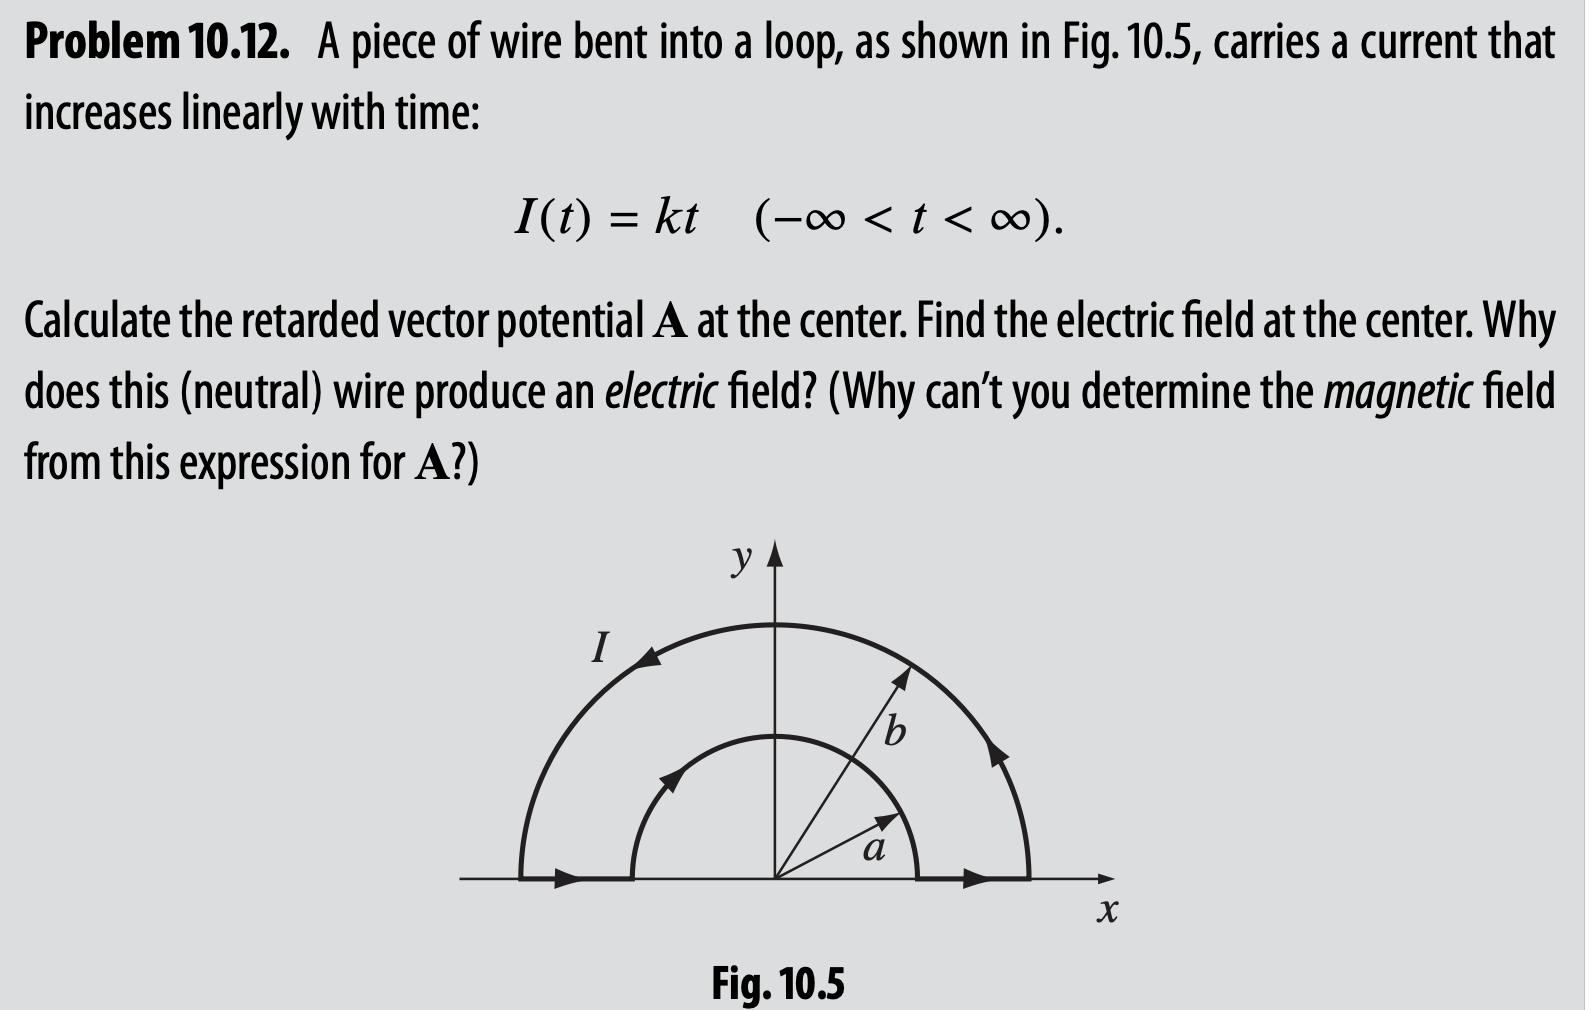
\includegraphics[width=0.8\textwidth]{Griffiths_prob_10_12.png}
\end{figure}

In general, the relevant one-dimensional integral is along the wire: \begin{align*}
    \mathbf{A}(\mathbf{r}, t) = \frac{\mu_0}{4 \pi } \int \frac{\mathbf{I}(\mathbf{r}^{\prime} , t_r)}{\griffr[2] } d l ^{\prime} 
\end{align*}

But the current only depends on time and not on position. Along the top wire we get \begin{align*}
    \mathbf{I}(t_r) = k(t - \frac{b}{c})\hat{\boldsymbol{\phi}} = (t - \frac{b}{c})\left[ - \sin \theta \hat{\mathbf{x}} + \cos \theta \hat{\mathbf{y}} \right] 
\end{align*}
while along the bottom we have \begin{align*}
    \mathbf{I}(t_r) = k(t - \frac{a}{c})(-\hat{\boldsymbol{\phi}}) = (t - \frac{a}{c})\left[ \sin \theta \hat{\mathbf{x}} - \cos \theta \hat{\mathbf{y}} \right] 
\end{align*}
such that from those contributions we get \begin{align*}
    \mathbf{A}_{\text{top and bottom}}(\mathbf{r}, t) = \frac{k\mu_0}{4 \pi } \biggl[ &\hat{\mathbf{x}} \int_0 ^\pi  d \theta \sin \theta \left( a\left( t- \frac{a}{c} \right) +  b\left(t - \frac{b}{c}\right) \right)\\
      &\hat{\mathbf{y}} \int_0 ^\pi d \theta \cos \theta \left( b \left( t - \frac{b}{c} \right) + a \left( t - \frac{a}{c} \right)   \right) \biggr]
\end{align*}
plenty of things are independent of \(\theta \) so we get \begin{align*}
    \mathbf{A}_{\text{top and bottom}}(\mathbf{r}, t) = \frac{k\mu_0}{2\pi } \left( t (a + b) -  \frac{1}{c}\left( a^{2} + b^{2}  \right) \right) 
\end{align*}
whereas from the horizontal segments we get (I think they will be equal, but the "doppler" effect would actually play in here with a point charge. This is why we have terms involving the velocity vector in that case. But here I think they should be the same in the sense that it is symmetrical w.r.t.\ time):
\begin{align*}
    \mathbf{A}_{\text{left horizontal}}(\mathbf{r}, t) &= \frac{k\mu_0}{4 \pi } \hat{\mathbf{x}} \int_b ^a \frac{t - \frac{x^{\prime}}{c} }{x^{\prime}} dx^{\prime} \\
    &=  \frac{k\mu_0}{4 \pi } \hat{\mathbf{x}} \left( t \ln \left(\frac{a}{b}\right) - \frac{a - b}{c} \right) 
\end{align*}
but of course with the right horizontal, we are integrating the exact same thing, but from \(a \to  b\). Thus they cancel. This seems wierd to me right now, since with the right hand rule from the current, I would think the field would have to contribute something. But I do see that the center is on the line of the two horizontal segments. But if we only had one side, that should prevent the field, right? I got a contribution from the left side alone. It was just cancelled by the right side it seems.  

\subsection*{Follow-Up Questions/Ideas/ToDos}
\begin{itemize}
    \item It seems weird that there can be different retarded times from the same field point to a point charge, but that's apparently necessary with classical electrodynamics. \textred{What's the full story?}
    \item In problem 10.12 above, it confuses me that flipping the limits of integration is the same as flipping the direction of the current in some sense. When we are running along the inner half circle (the one at radius \(a\)), I have the urge to say that it is running in the direction \(- \boldsymbol{\hat{\mathbf{\phi}}}\) while the angle being sweeped is from \(\pi \to 0\). But this is "a double flip" and leaves the integral unchanged. At the same time, I feel like the two horizontal wire segments shouldn't cancel. They are running in the same direction one would think. But with respect to the center point, they \textit{are} running in oppositse directions of course. \textred{Don't think so much about things where you can say: Of course it has to be this way. Of course you don't want to double flip, since you see that it leaves everything unchanged. Don't worry so much!}
\end{itemize}
